%==============================================================
%  DeepGuard AI — Final Year Project Report
%  Author : Mohamed Mbarek
%  Year   : 2025–2026
%  University : Faculté des Sciences de Gafsa
%==============================================================

\documentclass[12pt,a4paper,openany,oneside]{book}

% ---------- Load configuration ----------
%==============================================================
%  LaTeX Packages — Final clean version (with header fix)
%==============================================================

% ---------- Language & Encoding ----------
\usepackage[utf8]{inputenc}
\usepackage[T1]{fontenc}
\usepackage[english]{babel}
\usepackage{csquotes}            % Recommended by biblatex

% ---------- Fonts ----------
\usepackage{lmodern}             % Modern Latin font
\usepackage{charter}             % Clean serif font for body
\usepackage[scaled=0.9]{helvet}  % Sans-serif (Helvetica style)
\usepackage{courier}             % Monospace for code
\renewcommand{\familydefault}{\sfdefault} % Default to sans-serif (more modern)

% ---------- Page Layout ----------
\usepackage[a4paper,
            top=2.5cm,
            bottom=2.5cm,
            left=2.5cm,
            right=2.5cm,
            headheight=15pt]{geometry}

% ---------- Spacing ----------
\usepackage{setspace}
\onehalfspacing

% ---------- Colors ----------
\usepackage{xcolor}

% Brand colors (matching DeepGuard AI)
\definecolor{deepblue}{HTML}{1E40AF}      % Primary blue
\definecolor{deeppurple}{HTML}{7C3AED}    % Accent purple
\definecolor{deepdark}{HTML}{0F172A}      % Dark slate
\definecolor{deeplight}{HTML}{F1F5F9}     % Light gray
\definecolor{deepaccent}{HTML}{3B82F6}    % Light blue
\definecolor{codegray}{HTML}{F8FAFC}      % Code background

% Risk colors
\definecolor{riskgreen}{HTML}{22C55E}
\definecolor{riskyellow}{HTML}{EAB308}
\definecolor{riskorange}{HTML}{F97316}
\definecolor{riskred}{HTML}{EF4444}

% ---------- Graphics ----------
\usepackage{graphicx}
\graphicspath{{figures/}}
\usepackage{float}
\usepackage{wrapfig}
\usepackage{subcaption}

% ---------- Tables ----------
\usepackage{tabularx}
\usepackage{booktabs}
\usepackage{multirow}
\usepackage{multicol}
\usepackage{array}
\usepackage{longtable}
\usepackage{colortbl}

% ---------- Math ----------
\usepackage{amsmath}
\usepackage{amssymb}
\usepackage{amsfonts}

% ---------- Lists ----------
\usepackage{enumitem}
\setlist{itemsep=2pt, topsep=4pt}

% ---------- Hyperlinks ----------
\usepackage[hidelinks,
            colorlinks=true,
            linkcolor=deepblue,
            citecolor=deeppurple,
            urlcolor=deepaccent,
            bookmarksnumbered=true]{hyperref}

% ---------- Headers & Footers ----------
\usepackage{fancyhdr}
\pagestyle{fancy}
\fancyhf{}
\fancyhead[L]{\nouppercase{\leftmark}}
\fancyhead[R]{\thepage}
\renewcommand{\headrulewidth}{0.4pt}
\renewcommand{\footrulewidth}{0pt}

%==============================================================
%  HEADER FIX: Update \chaptermark for unnumbered chapters
%  This fixes the bug where General Conclusion showed
%  "Chapter 5. Testing and Validation" as the header
%==============================================================
\makeatletter

% For numbered chapters (\chapter): show "Chapter X. Title"
\renewcommand{\chaptermark}[1]{%
  \markboth{Chapter \thechapter.\ #1}{}}

% Custom command for unnumbered chapters (\chapter*): show just the title
\newcommand{\setunnumberedchapter}[1]{%
  \markboth{#1}{}}

%==============================================================
%  Custom Chapter Style (native LaTeX — no titlesec, no warnings)
%==============================================================

% Numbered chapter style — used by \chapter
\def\@makechapterhead#1{%
  \vspace*{20pt}%
  {\parindent \z@ \raggedright \normalfont
   \sffamily\Large\bfseries\color{deeppurple}
   Chapter \thechapter
   \par\nobreak
   \vskip 6pt
   {\color{deepblue}\rule{\textwidth}{1.5pt}}
   \par\nobreak
   \vskip 12pt
   \huge\bfseries\color{deepblue} #1
   \par\nobreak
   \vskip 6pt
   {\color{deepblue}\rule{\textwidth}{0.5pt}}
   \par\nobreak
   \vskip 30pt
  }}

% Unnumbered chapter style — used by \chapter*
% Now also updates the header so it doesn't show old chapter info
\def\@makeschapterhead#1{%
  \markboth{#1}{}%
  \vspace*{20pt}%
  {\parindent \z@ \raggedright \normalfont
   \sffamily
   {\color{deepblue}\rule{\textwidth}{1.5pt}}
   \par\nobreak
   \vskip 12pt
   \huge\bfseries\color{deepblue} #1
   \par\nobreak
   \vskip 6pt
   {\color{deepblue}\rule{\textwidth}{0.5pt}}
   \par\nobreak
   \vskip 30pt
  }}

%==============================================================
%  Custom Section Style (native — replaces sectsty, no warnings)
%==============================================================
\renewcommand{\section}{%
  \@startsection{section}{1}{0pt}%
    {-3.5ex \@plus -1ex \@minus -.2ex}%
    {2.3ex \@plus.2ex}%
    {\normalfont\sffamily\Large\bfseries\color{deepblue}}%
}

\renewcommand{\subsection}{%
  \@startsection{subsection}{2}{0pt}%
    {-3.25ex\@plus -1ex \@minus -.2ex}%
    {1.5ex \@plus .2ex}%
    {\normalfont\sffamily\large\bfseries\color{deepdark}}%
}

\renewcommand{\subsubsection}{%
  \@startsection{subsubsection}{3}{0pt}%
    {-3.25ex\@plus -1ex \@minus -.2ex}%
    {1.5ex \@plus .2ex}%
    {\normalfont\sffamily\normalsize\bfseries\color{deepdark}}%
}

\makeatother

% ---------- Code Listings ----------
\usepackage{listings}

\lstdefinestyle{mystyle}{
    backgroundcolor=\color{codegray},
    commentstyle=\color{gray}\itshape,
    keywordstyle=\color{deepblue}\bfseries,
    numberstyle=\tiny\color{gray},
    stringstyle=\color{deeppurple},
    basicstyle=\ttfamily\footnotesize,
    breakatwhitespace=false,
    breaklines=true,
    captionpos=b,
    keepspaces=true,
    numbers=left,
    numbersep=5pt,
    showspaces=false,
    showstringspaces=false,
    showtabs=false,
    tabsize=2,
    frame=single,
    rulecolor=\color{deepaccent},
    framesep=4pt,
    xleftmargin=15pt
}
\lstset{style=mystyle}

% ---------- Tikz for diagrams (optional) ----------
\usepackage{tikz}
\usetikzlibrary{shapes.geometric, arrows, positioning, fit, calc}

% ---------- Quote environment ----------
\usepackage{epigraph}
\setlength{\epigraphwidth}{0.6\textwidth}

% ---------- Bibliography ----------
\usepackage[backend=biber,
            style=ieee,
            sorting=none]{biblatex}

% Force biblatex to print all references in the .bib file
% (so the bibliography section is not empty during template phase)
% --> This line will be REMOVED once we cite references in real chapters
\nocite{*}

% ---------- Misc ----------
\usepackage{lipsum}              % For placeholder text only
\usepackage{lastpage}
\usepackage{afterpage}

%==============================================================
%  Document Settings
%==============================================================

% ---------- Paragraph Settings ----------
\setlength{\parindent}{0pt}
\setlength{\parskip}{8pt}

% ---------- Caption Style ----------
\usepackage{caption}
\captionsetup{
    font={small,it},
    labelfont={bf,color=deepblue},
    labelsep=colon,
    justification=centering
}

% ---------- Custom Box for Highlighted Text ----------
\usepackage[most]{tcolorbox}

\newtcolorbox{infobox}[1][]{
    colback=deeplight,
    colframe=deepblue,
    fonttitle=\bfseries,
    arc=2mm,
    boxrule=1pt,
    left=8pt, right=8pt, top=6pt, bottom=6pt,
    #1
}

\newtcolorbox{warningbox}[1][]{
    colback=yellow!10,
    colframe=riskorange,
    fonttitle=\bfseries,
    arc=2mm,
    boxrule=1pt,
    left=8pt, right=8pt, top=6pt, bottom=6pt,
    #1
}

\newtcolorbox{notebox}[1][]{
    colback=blue!5,
    colframe=deepaccent,
    fonttitle=\bfseries,
    arc=2mm,
    boxrule=1pt,
    left=8pt, right=8pt, top=6pt, bottom=6pt,
    #1
}

% ---------- Custom Tabular ----------
\renewcommand{\arraystretch}{1.3}

% ---------- Toc Style ----------
\usepackage{tocloft}
\renewcommand{\cftchapfont}{\bfseries\color{deepblue}}
\renewcommand{\cftsecfont}{\color{deepdark}}
\renewcommand{\cftchappagefont}{\bfseries\color{deepblue}}

% ---------- Disable widow & orphan lines ----------
\widowpenalty=10000
\clubpenalty=10000

% ---------- Better line breaking ----------
\sloppy

%==============================================================
%  Custom Commands & Shortcuts
%==============================================================

% Project name shortcut
\newcommand{\deepguard}{\textbf{DeepGuard AI}}
\newcommand{\projectname}{DeepGuard AI}

% Inline code
\newcommand{\code}[1]{\texttt{\textcolor{deepblue}{#1}}}

% Tech name highlight (Python, FastAPI, etc.)
\newcommand{\tech}[1]{\textbf{\textcolor{deeppurple}{#1}}}

% Bold blue keyword
\newcommand{\keyword}[1]{\textbf{\textcolor{deepblue}{#1}}}

% Figure helper (simplifies inserting figures)
\newcommand{\addfigure}[3]{%
    \begin{figure}[H]
        \centering
        \includegraphics[width=#2\textwidth]{#1}
        \caption{#3}
        \label{fig:#1}
    \end{figure}
}

% Placeholder for missing figures
\newcommand{\placeholderfig}[2]{%
    \begin{figure}[H]
        \centering
        \fbox{\parbox[c][6cm][c]{0.8\textwidth}{%
            \centering\Large\textcolor{gray}{[Figure Placeholder]}\\
            \normalsize\textcolor{gray}{#1}
        }}
        \caption{#2}
    \end{figure}
}


% ---------- Bibliography ----------
\addbibresource{references.bib}

%==============================================================
%  Toggle empty front matter sections
%  Set to true once you have figures/tables to display
%==============================================================
\newif\ifshowfigureslist
\newif\ifshowtableslist
\showfigureslistfalse  % Set to \showfigureslisttrue when you have figures
\showtableslistfalse   % Set to \showtableslisttrue when you have tables

\begin{document}

% =============== FRONT MATTER ===============
\frontmatter
\pagestyle{plain}

%==============================================================
%  Cover Page — Official University Template (English version)
%  University logo: 3cm height
%  Header minipages: CENTER-aligned [c] (fixes baseline overflow)
%==============================================================

\begin{titlepage}
    \pagecolor{white}

    % Top decorative bar
    \begin{tikzpicture}[remember picture, overlay]
        \fill[deepblue] (current page.north west) rectangle ([yshift=-0.7cm]current page.north east);
        \fill[deeppurple] ([yshift=-0.7cm]current page.north west) rectangle ([yshift=-0.85cm]current page.north east);
    \end{tikzpicture}

    \vspace*{0cm}

    %---------- Three-column institutional header (CENTER-aligned) ----------
    % LEFT text | CENTER University logo | RIGHT text
    \noindent
    \begin{minipage}[c]{0.34\textwidth}
        \centering\scriptsize
        \textbf{Republic of Tunisia}\\
        Ministry of Higher Education\\
        and Scientific Research\\
        \textbf{University of Gafsa}
    \end{minipage}
    \hfill
    \begin{minipage}[c]{0.28\textwidth}
        \centering
        % University of Gafsa logo (real image)
        \includegraphics[height=3cm]{logo_university.png}
    \end{minipage}
    \hfill
    \begin{minipage}[c]{0.34\textwidth}
        \centering\scriptsize
        \textbf{Faculty of Sciences of Gafsa}\\
        \textbf{Department of Computer Science}\\
        Final Year Project\\
        Order N°: PFE-2026/.......
    \end{minipage}

    \vspace{0.15cm}

    % Horizontal separator (blue line)
    {\color{deepblue}\rule{\textwidth}{0.8pt}}

    \vspace{0.15cm}

    %---------- Department of Computer Science logo (real image, centered) ----------
    \begin{center}
        \includegraphics[height=1.3cm]{logo_department.png}
    \end{center}

    \vspace{0.15cm}

    %---------- Main title (compact) ----------
    \begin{center}
        {\large\bfseries FINAL YEAR PROJECT REPORT}\\[2pt]
        {\footnotesize\itshape Submitted to}\\[1pt]
        {\small\bfseries Faculty of Sciences of Gafsa}\\[1pt]
        {\footnotesize\itshape In partial fulfillment of the requirements for the}\\[2pt]
        {\small\bfseries BACHELOR'S DEGREE IN COMPUTER SCIENCE:}\\[1pt]
        {\small\bfseries SOFTWARE ENGINEERING AND INFORMATION SYSTEMS}
    \end{center}

    \vspace{0.15cm}

    %---------- Project title block (between two lines) ----------
    {\color{deepblue}\rule{\textwidth}{1pt}}
    \begin{center}
        \vspace{3pt}
        {\huge\bfseries\textcolor{deepdark}{DeepGuard AI}}\\[2pt]
        {\normalsize\textcolor{deepblue}{\itshape An AI-Powered Deepfake Detection}}\\[1pt]
        {\normalsize\textcolor{deepblue}{\itshape and Digital Forensics Platform}}
        \vspace{3pt}
    \end{center}
    {\color{deepblue}\rule{\textwidth}{1pt}}

    \vspace{0.2cm}

    %---------- Presented by ----------
    \begin{center}
        {\footnotesize\bfseries Presented by:}\\[1pt]
        {\normalsize\bfseries Mohamed Mbarek}
    \end{center}

    \vspace{0.15cm}

    %---------- Jury ----------
    \begin{center}
        {\footnotesize\itshape Defended on \dotfill/\dotfill/\dotfill\ before the jury composed of:}
    \end{center}

    \vspace{2pt}

    \begin{center}
    \renewcommand{\arraystretch}{1.0}
    \small
    \begin{tabular}{p{5.5cm} p{5.5cm}}
        \textbf{Mr./Mrs.} \dotfill           & \textbf{President}    \\
        \textbf{Mr./Mrs.} \dotfill           & \textbf{Examiner}     \\
        \textbf{Mr. Othmani Mohamed}         & \textbf{Supervisor}   \\
    \end{tabular}
    \end{center}

    \vspace{0.3cm}

    %---------- Academic year (our modern style) ----------
    \begin{center}
    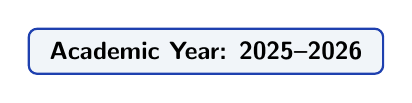
\begin{tikzpicture}
        \node[rectangle, draw=deepblue, line width=0.8pt, rounded corners=3pt,
              fill=deeplight, inner sep=5pt, minimum width=4.5cm]
              {\small\textbf{Academic Year: 2025--2026}};
    \end{tikzpicture}
    \end{center}

    \vfill

    % Bottom decorative bar
    \begin{tikzpicture}[remember picture, overlay]
        \fill[deeppurple] ([yshift=0.85cm]current page.south west) rectangle ([yshift=0.7cm]current page.south east);
        \fill[deepblue] ([yshift=0.7cm]current page.south west) rectangle (current page.south east);
    \end{tikzpicture}

\end{titlepage}

\nopagecolor

%---------- Page numbering ----------
\setcounter{page}{1}
%==============================================================
%  Dedication Page — Right-aligned, classic style
%  This page is intentionally unnumbered (decorative page)
%  Counter is rolled back so the next page (Acknowledgments) = "i"
%==============================================================

\clearpage
\thispagestyle{empty}

\vspace*{\fill}

\begin{center}
    {\Huge\itshape\color{deepblue} Dedication}
\end{center}

\vspace{1.5cm}

\begin{flushright}
\begin{minipage}{0.7\textwidth}
\itshape
\setstretch{1.3}
\begin{flushright}

\textit{To my beloved parents,}\\
whose endless love, patience, and sacrifices\\
made every step of this journey possible.\\[14pt]

\textit{To my family,}\\
for their continuous encouragement\\
and unwavering belief in me.\\[14pt]

\textit{To my friends,}\\
who shared the long nights, the struggles,\\
and the small victories along the way.\\[14pt]

\textit{To my teachers and supervisor,}\\
who guided me with their knowledge,\\
patience, and trust.\\[14pt]

\textit{And to everyone who supported me,}\\
even with a single word of encouragement.\\[24pt]

\textbf{Thank you.}\\[6pt]
\textit{— Mohamed Mbarek}

\end{flushright}
\end{minipage}
\end{flushright}

\vspace*{\fill}

% Roll back the page counter so this page doesn't count.
% Result: next page (Acknowledgments) starts at "i".
\addtocounter{page}{-1}

%==============================================================
%  Acknowledgments Page
%==============================================================

\cleardoublepage
\thispagestyle{empty}

\chapter*{Acknowledgments}
\addcontentsline{toc}{chapter}{Acknowledgments}

\setstretch{1.4}

I would like to begin by expressing my sincere gratitude to everyone who contributed, directly or indirectly, to the completion of this final year project.

\vspace{5pt}

First and foremost, I would like to thank my supervisor, \textbf{Mr.~Othmani Mohamed}, for his valuable guidance, constructive feedback, and continuous availability throughout the development of this work. His advice and encouragement played a key role in shaping the direction of this project.

\vspace{5pt}

I also wish to extend my appreciation to all the teachers of the \textbf{Faculty of Sciences of Gafsa}, who shared their knowledge and experience with us during these years of study. Their dedication helped build the technical foundation that made a project of this scale possible.

\vspace{5pt}

A special thanks goes to the members of the jury, who kindly accepted to evaluate this work. I am honored by their time and attention.

\vspace{5pt}

I am deeply grateful to my parents and family for their unconditional support, patience, and constant encouragement throughout my entire academic journey. Their belief in me has been the strongest motivation.

\vspace{5pt}

Finally, I would like to thank my friends and classmates for the moments of collaboration, discussion, and mutual support that made this experience much more meaningful.

\vspace{10pt}

\begin{flushright}
\textit{Mohamed Mbarek}
\end{flushright}

%==============================================================
%  Abstract Page (English + French Résumé)
%==============================================================

\cleardoublepage
\thispagestyle{empty}

\chapter*{Abstract}
\addcontentsline{toc}{chapter}{Abstract}

\setstretch{1.4}

The rapid advancement of generative artificial intelligence has made the creation of highly realistic synthetic media — known as \textit{deepfakes} — accessible to anyone. While the technology has legitimate creative uses, it has also become a serious threat to digital trust, journalism, and personal identity. Detecting manipulated media is no longer optional; it is a necessity.

\vspace{5pt}

This project, titled \textbf{\projectname}, presents a complete web-based platform for detecting deepfakes in images and videos and producing professional digital forensics reports. The system combines a Vision Transformer (ViT) model from Hugging Face with face detection (MTCNN), image normalization techniques, EXIF metadata analysis, and a clean user interface built with React and Tailwind CSS. The backend, powered by FastAPI and PostgreSQL, exposes a secured REST API protected by JWT authentication.

\vspace{5pt}

The platform offers several features designed for real-world use: image and video analysis, risk scoring (0--100), forensic metadata inspection, PDF report generation, shareable result links, and a personal dashboard with scan history. The development followed the \textbf{2TUP (Two Track Unified Process)} methodology, which separates functional and technical concerns and proved well suited to a solo academic project of this scope.

\vspace{5pt}

The final system demonstrates that effective deepfake detection can be combined with explainability and forensics in a single, user-friendly application — providing a practical tool for journalists, researchers, and the general public.

\vspace{10pt}

\noindent\textbf{Keywords:} Deepfake detection, Artificial Intelligence, Vision Transformer, Digital Forensics, EXIF Metadata, FastAPI, React, JWT Authentication, Cybersecurity, Media Authenticity.

\newpage

% ---------- French Résumé ----------
\addcontentsline{toc}{chapter}{Résumé}
\begin{center}
\rule{0.4\textwidth}{0.4pt}
\end{center}

\noindent\textbf{\large Résumé}

\vspace{8pt}

L'évolution rapide de l'intelligence artificielle générative a rendu la création de médias synthétiques très réalistes — appelés \textit{deepfakes} — accessible à tous. Bien que cette technologie ait des usages créatifs légitimes, elle est également devenue une menace sérieuse pour la confiance numérique, le journalisme et l'identité personnelle. La détection des médias manipulés n'est plus une option, c'est une nécessité.

\vspace{5pt}

Ce projet, intitulé \textbf{\projectname}, présente une plateforme web complète pour la détection de deepfakes dans les images et les vidéos, ainsi que la génération de rapports professionnels d'analyse forensique. Le système combine un modèle Vision Transformer (ViT) issu de Hugging Face avec la détection de visages (MTCNN), des techniques de normalisation d'images, l'analyse des métadonnées EXIF, et une interface utilisateur moderne développée avec React et Tailwind CSS. Le backend, propulsé par FastAPI et PostgreSQL, expose une API REST sécurisée par authentification JWT.

\vspace{5pt}

La plateforme propose plusieurs fonctionnalités pensées pour un usage réel : analyse d'images et de vidéos, score de risque (0--100), inspection des métadonnées forensiques, génération de rapports PDF, liens de résultats partageables, et un tableau de bord personnel avec historique des analyses. Le développement a suivi la méthodologie \textbf{2TUP (Two Track Unified Process)}, qui sépare les préoccupations fonctionnelles et techniques et s'est révélée bien adaptée à un projet académique individuel de cette envergure.

\vspace{5pt}

Le système final démontre que la détection efficace des deepfakes peut être combinée avec l'explicabilité et l'analyse forensique au sein d'une seule application conviviale — offrant un outil pratique pour les journalistes, les chercheurs et le grand public.

\vspace{10pt}

\noindent\textbf{Mots-clés :} Détection de deepfake, Intelligence Artificielle, Vision Transformer, Analyse Forensique, Métadonnées EXIF, FastAPI, React, Authentification JWT, Cybersécurité, Authenticité des Médias.

% Table of contents
\clearpage
\pdfbookmark[0]{Table of Contents}{toc}
\tableofcontents

% List of Figures (only if enabled)
\ifshowfigureslist
    \clearpage
    \listoffigures
    \addcontentsline{toc}{chapter}{List of Figures}
\fi

% List of Tables (only if enabled)
\ifshowtableslist
    \clearpage
    \listoftables
    \addcontentsline{toc}{chapter}{List of Tables}
\fi

% =============== MAIN MATTER ===============
\mainmatter
\pagestyle{fancy}

% General Introduction
\chapter*{General Introduction}
\addcontentsline{toc}{chapter}{General Introduction}
%==============================================================
%  General Introduction
%==============================================================

For most of modern history, a photograph or a video served as a kind of evidence. If something appeared on a screen, the assumption was that someone, somewhere, had captured it with a camera. That assumption is now harder to defend. The same artificial intelligence that produces remarkable creative tools is also producing convincing synthetic images and videos of people who never said or did the things attributed to them. The shift has been quiet but rapid, and its consequences are still being measured.

The term \textit{deepfake} entered public awareness around 2017, when an anonymous developer used a deep learning technique called Generative Adversarial Networks to swap faces in videos. What started as a curiosity on online forums quickly evolved into a category of content that millions of people now encounter without realizing it. Today, free or cheap tools can replace a face in a video, clone a voice from a short audio sample, or generate an entirely synthetic portrait that looks like a real person. The barrier to entry has effectively collapsed. The applications range from harmless entertainment to deliberate disinformation, with documented cases in journalism, politics, finance, and personal identity theft.

Detecting manipulated media is, in principle, the natural counter-response. In practice it has turned out to be one of the harder problems in modern computer vision. The latest generative models produce results that the human eye genuinely cannot distinguish from real photographs in most viewing conditions. Specialized detection tools do exist, but they tend to be commercial products aimed at governments and large media organizations, with prices and access restrictions that put them out of reach of journalists, researchers, students, and ordinary citizens who arguably need them the most.

This thesis presents \deepguard{}, a final year project carried out at the Faculty of Sciences of Gafsa, in partial fulfillment of the requirements for the Bachelor's degree in Computer Science (Software Engineering and Information Systems). The platform offers a complete pipeline for analyzing images and videos, returning a clear verdict on their authenticity, and producing a forensic report that can be downloaded, shared, or consulted directly through a personal dashboard. The goal is not to compete with the commercial solutions mentioned above, but to demonstrate that a working, accessible, and well-engineered alternative can be built within the scope of an academic project.

The development followed the 2TUP (Two Track Unified Process) methodology, which separates the analysis of a software project into two parallel tracks --- one focused on what the system should do, the other on how it should be built --- and merges them into a unified architecture at the end. The choice was deliberate. It suits a solo developer better than team-based approaches such as Scrum, and it reflects naturally in the structure of the chapters that follow.

The report is organized into five chapters.\\[6pt]
\textbf{Chapter 1} sets the general context, surveys existing detection tools, and presents the methodology and timeline of the project.\\[6pt]
\textbf{Chapter 2} follows the functional track of 2TUP, identifying the actors, capturing the functional and non-functional requirements, and modeling the expected behavior of the system through use case and sequence diagrams.\\[6pt]
\textbf{Chapter 3} covers the technical track and the merge phase, justifying the technology choices and describing the global architecture, the database design, the REST API, and the AI detection pipeline.\\[6pt]
\textbf{Chapter 4} presents the implementation itself, with code structure explanations and screenshots of the finished application.\\[6pt]
\textbf{Chapter 5} reports on the testing campaign, covering AI model accuracy, functional tests, edge cases, and security checks.\\[6pt]
A \textbf{General Conclusion} closes the report by summarizing what was achieved and discussing possible future improvements.

% Chapters
%==============================================================
%  Chapter 1 — General Context
%==============================================================

\chapter{General Context}
\label{chap:context}

\textit{This first chapter sets the stage for the entire project. It explains the broader context in which the work takes place, defines the problem that motivated it, examines what already exists on the market, and introduces the proposed solution. The chapter also presents the methodology that guided the development process and outlines the overall timeline.}

\vspace{1cm}

%==============================================================
\section{Introduction}
%==============================================================

Artificial intelligence has progressed at a pace that very few people anticipated even five years ago. Tools that once required research labs and expensive hardware can now be installed on a laptop and used by anyone with basic computer skills. This shift has opened the door to many positive applications, but it has also given rise to new categories of risk. One of the most discussed of these risks is the deepfake: a synthetic image or video, generated or manipulated by AI, that imitates a real person convincingly enough to mislead the average viewer.

The work presented in this report responds to that specific problem. It introduces \deepguard{}, a web-based platform that uses modern computer vision techniques to determine whether an uploaded image or video is genuine or has been generated or altered by AI. Beyond a simple verdict, the platform produces a detailed forensic analysis that the user can consult, share, or download as a professional report. This chapter prepares the ground for everything that follows: it describes the problem, surveys what existing tools offer, and explains why a new approach was worth building.

%==============================================================
\section{Project Context}
%==============================================================

The last few years have seen a noticeable acceleration in generative AI technologies. Models capable of creating realistic faces, synthetic voices, and full video sequences have moved from research papers into open-source repositories and consumer applications. Tools such as Stable Diffusion, Midjourney, and various face-swap programs are now widely available, often free of charge, and require very little technical background to operate. As a direct result, the cost and effort required to produce convincing synthetic media have collapsed.

This democratization is, in many ways, a positive development. Filmmakers experiment with new visual effects, educators recreate historical scenes, and small businesses generate marketing material without large budgets. But the same tools also make it easier to fabricate evidence, impersonate public figures, and circulate false information that looks visually authentic. Journalists, lawyers, and even ordinary social media users now face a question that did not really exist a decade ago: \textit{can I still trust what I see on a screen?}

From an academic perspective, the topic sits at an interesting crossroads between several fields: computer vision, cybersecurity, digital forensics, and software engineering. It also has an unmistakable social dimension, since the spread of manipulated media touches issues of trust, politics, and personal reputation. These combined factors made the subject a natural fit for a final year project in software engineering, where both the technical depth and the real-world relevance were strong enough to justify a complete platform rather than a small prototype.

%==============================================================
\section{Problem Statement}
%==============================================================

The central problem is straightforward to describe but difficult to solve in practice. Given a piece of digital content, usually an image or a short video, how can a user reliably determine whether it shows a real human face or a synthetic one? The challenge is no longer purely visual. Modern deepfakes can fool the human eye, and even experienced viewers admit that distinguishing real from fake media has become nearly impossible without technical assistance.

Several concrete situations illustrate why this matters. A news outlet receiving a leaked video of a politician must verify its authenticity before publishing. A recruiter conducting a remote interview wants to be sure that the candidate on the screen is genuinely the person being hired. A bank reviewing a video-based identity check needs to detect any attempt to impersonate a client. In each of these cases, the cost of being wrong is significant, ranging from reputational damage to financial loss to legal consequences.

The problem becomes harder when the analysis must remain accessible to non-experts. A solution that requires installing complex Python libraries, configuring GPUs, or interpreting raw model outputs would not help most of the people who actually need it. What is needed is a tool that can be used by a journalist, a teacher, or a curious citizen, with results presented clearly and supported by evidence that the user can understand.

%==============================================================
\section{Study of Existing Solutions}
%==============================================================

Several deepfake detection tools already exist on the market, each with a different focus and different limitations. Before designing \projectname{}, a study of these existing solutions was carried out to understand what works well and where current platforms fall short.

\textbf{Deepware Scanner} is a free online tool that allows users to upload videos and receive a probability score indicating whether the content is a deepfake. It is one of the most accessible solutions for the general public, but the analysis is limited to videos and does not include any forensic metadata inspection or detailed reporting.

\textbf{Sensity AI} is a commercial platform aimed at enterprises and government agencies. It offers high accuracy and continuous monitoring features, but it is closed-source, expensive, and not available to individual users or small organizations. Its detailed reports are also locked behind a paywall.

\textbf{Intel FakeCatcher} is a real-time deepfake detector developed by Intel. It uses an interesting biological signal called photoplethysmography, which measures subtle changes in blood flow visible in human skin. While the approach is innovative, the technology is not openly available and requires Intel-specific hardware to run efficiently.

\textbf{Microsoft Video Authenticator} was developed during the 2020 U.S. presidential election to help fight disinformation. It provides a confidence score for videos and images but has been distributed only to selected media partners, which makes it inaccessible to most users.

Table~\ref{tab:existing-solutions} summarizes the main strengths and weaknesses of each of these tools compared to the goals of this project.

\begin{table}[H]
\centering
\renewcommand{\arraystretch}{1.4}
\setlength{\tabcolsep}{6pt}
\begin{tabularx}{\textwidth}{|>{\bfseries}l|X|X|}
\hline
\rowcolor{deeplight}
\textbf{Solution} & \textbf{Strengths} & \textbf{Limitations} \\
\hline
Deepware Scanner & Free, simple interface, no installation & Videos only, no forensics, no reports \\
\hline
Sensity AI & High accuracy, enterprise-grade & Closed-source, expensive, not for individuals \\
\hline
Intel FakeCatcher & Innovative biological signal approach & Not publicly available, hardware-dependent \\
\hline
Microsoft Video Authenticator & Backed by Microsoft research & Distribution restricted to media partners \\
\hline
\rowcolor{deeplight}
\textbf{\projectname{}} & \textbf{Free, open, complete forensics, reports, sharing} & \textbf{Academic project, faces only (for now)} \\
\hline
\end{tabularx}
\caption{Comparison of existing deepfake detection solutions.}
\label{tab:existing-solutions}
\end{table}

Two main gaps emerge from this comparison. First, no single tool combines deepfake detection with full digital forensics in an accessible interface. Second, the most powerful systems are either locked behind commercial licenses or restricted to selected partners, leaving the general public without a reliable option. These gaps justified the development of a new solution.

%==============================================================
\section{Proposed Solution}
%==============================================================

The solution proposed in this project is \deepguard{}, a complete web platform that combines artificial intelligence and digital forensics in a single tool. The objective is not to compete with billion-dollar commercial products, but rather to demonstrate that a well-designed academic project can offer features that real users actually need, in a clean and accessible format.

At its core, \projectname{} uses a Vision Transformer model (ViT) fine-tuned on real and synthetic face data. The model is paired with a face detection step (MTCNN) so that the analysis focuses precisely on the regions that matter. For videos, frames are extracted at regular intervals and analyzed one by one, then aggregated into a single risk score on a scale from 0 to 100. The result is a clear verdict (real or fake) accompanied by a confidence percentage, a forensic report, and a downloadable PDF.

What distinguishes \projectname{} from most existing tools is the integration of digital forensics into the same workflow. When an image is uploaded, the system also reads its EXIF metadata, checks for traces of editing software such as Photoshop or Midjourney, and flags suspicious patterns like missing camera information or unusual timestamps. This additional layer of analysis gives the user more than just a score; it gives them evidence they can interpret and trust.

Finally, the entire experience is designed around usability. A modern interface built with React and Tailwind CSS allows users to drag and drop their files, see real-time progress, browse their scan history, switch between light and dark themes, and share results through a public link. These features make the platform suitable for journalists, researchers, students, and any user who needs a fast and credible second opinion on a piece of media.

%==============================================================
\section{Project Objectives}
%==============================================================

The project pursues a clear set of objectives, each chosen to address one specific aspect of the overall problem. They can be summarized as follows:

\begin{enumerate}[leftmargin=*, label=\textbf{\arabic*.}]
    \item Build a deepfake detection engine capable of analyzing both images and videos with a high level of accuracy.
    \item Implement a risk scoring system that translates raw model outputs into a clear, four-level verdict that any user can understand.
    \item Integrate a digital forensics module that extracts EXIF metadata and flags signs of AI generation or manual editing.
    \item Develop a secure backend with user authentication so that personal data and scan history remain isolated and protected.
    \item Design a modern, responsive web interface that supports drag-and-drop uploads, real-time feedback, and a dark mode.
    \item Generate professional PDF reports and shareable result links so that the analysis can be communicated easily outside the platform.
    \item Follow a clean, documented software engineering process that produces maintainable code and a system that can be extended in the future.
\end{enumerate}

These objectives also serve as the criteria against which the final result will be evaluated in Chapter~\ref{chap:testing}.

%==============================================================
\section{Methodology --- 2TUP}
%==============================================================

Choosing the right methodology was an important decision early in the project. Agile methods such as Scrum are popular in industry, but they are designed for teams of several people who can split work across roles. Because this project was carried out alone, a methodology that fits a solo developer was needed, while still providing the structure and documentation expected from a final year report.

The selected approach is \textbf{2TUP} (\textit{Two Track Unified Process}), a UML-based methodology proposed by Hubert Tardieu and widely used in academic engineering projects~\cite{tardieu2002}. Its main idea is to separate the analysis of a project into two parallel tracks that progress independently before being merged at the end. This separation between \textit{what} the system should do and \textit{how} it should be built makes the design phase clearer and reduces the risk of mixing functional decisions with technical ones too early.

The \textbf{functional track} concentrates on the user-facing side of the project. It identifies the actors, captures the functional and non-functional requirements, models the use cases, and produces the UML diagrams that describe the expected behavior of the system. In other words, it answers the question: \textit{what does the user need from this platform?}

The \textbf{technical track} runs in parallel and focuses on the implementation side. It evaluates the technologies available, decides which architecture is most appropriate, and produces the technical models such as the class diagram, the database schema, and the API design. Its guiding question is: \textit{which tools and structures will deliver the required behavior?}

Once both tracks have reached a sufficient level of detail, they enter the \textbf{merge phase}. At this point, the functional and technical decisions are combined into a unified general architecture, which then drives the actual implementation and testing of the system. This logical separation followed by a controlled merge proved well suited to the scope of \projectname{}, and it is reflected directly in the structure of the next chapters: Chapter~\ref{chap:analysis} covers the functional track, Chapter~\ref{chap:design} covers the technical track and the merge phase, and Chapter~\ref{chap:implementation} presents the realization phase that follows.

%==============================================================
\section{Development Plan}
%==============================================================

The development of \projectname{} was spread over four months, which is a realistic duration for a project of this scope when carried out by a single student. The work was divided into four main phases, each with a clear focus, although in practice the boundaries between them were never strictly fixed. Table~\ref{tab:gantt} presents the overall plan in a simplified Gantt-chart format.

\begin{table}[H]
\centering
\renewcommand{\arraystretch}{1.4}
\setlength{\tabcolsep}{8pt}
\begin{tabularx}{\textwidth}{|>{\bfseries}l|X|c|c|c|c|}
\hline
\rowcolor{deeplight}
\textbf{Phase} & \textbf{Main Activities} & \textbf{M1} & \textbf{M2} & \textbf{M3} & \textbf{M4} \\
\hline
Research \& Setup &
Literature review, study of existing tools, technology choices, environment setup, initial AI model testing
& \cellcolor{deepaccent} & & & \\
\hline
Core AI \& Backend &
Preprocessing pipeline, face detection, risk scoring, FastAPI backend, database design, JWT authentication
& \cellcolor{deepaccent} & \cellcolor{deepaccent} & & \\
\hline
Frontend \& Integration &
React frontend (all pages), API integration, dashboard, history, forensics module, theme system
& & \cellcolor{deepaccent} & \cellcolor{deepaccent} & \\
\hline
Polish, Testing \& Defense &
PDF reports, share links, edge case handling, full testing campaign, thesis writing, defense preparation
& & & \cellcolor{deepaccent} & \cellcolor{deepaccent} \\
\hline
\end{tabularx}
\caption{Simplified Gantt chart of the project (M1--M4 = months 1 to 4).}
\label{tab:gantt}
\end{table}

The first month was mostly exploratory. A significant amount of time went into reading documentation, comparing existing solutions, and testing pre-trained models to confirm that a usable accuracy could be reached without training a model from scratch. The second and third months were the most intense, with most of the AI pipeline, the backend, and the frontend being built during this period. The final month was reserved for polishing, edge case handling, the full testing campaign, and the writing of this report.

%==============================================================
\section{Conclusion}
%==============================================================

This chapter has introduced the broader context of the project, explained the problem it tries to solve, examined what existing tools currently offer, and presented \deepguard{} as a complete and accessible alternative. The objectives have been clearly stated, and the chosen methodology (2TUP) and overall timeline have been described. The next chapter takes the first concrete step into the project itself by following the functional track of 2TUP: identifying the actors, capturing the requirements, and modeling the expected behavior of the system through UML diagrams.

%==============================================================
%  Chapter 2 — Requirements and Analysis
%==============================================================

\chapter{Requirements and Analysis}
\label{chap:analysis}

\textit{This chapter follows the functional track of the 2TUP methodology. It identifies the actors, the functional and non-functional requirements, and presents the UML diagrams that describe the expected behavior of the system.}

\vspace{1cm}

\section{Introduction}
\lipsum[1]

\section{Identification of Actors}
\lipsum[2]

\section{Functional Requirements}
\lipsum[3]

\section{Non-Functional Requirements}
\lipsum[4]

\section{Use Case Diagram}
\lipsum[5]

\section{Detailed Use Cases}
\lipsum[6]

\section{Sequence Diagrams}
\lipsum[7]

\section{Conclusion}
\lipsum[8]

%==============================================================
%  Chapter 3 — Architecture and Technical Design
%==============================================================

\chapter{Architecture and Technical Design}
\label{chap:design}

\textit{This chapter follows the technical track and the merge phase of the 2TUP methodology. It justifies the technology choices, describes the system architecture, the database schema, the AI pipeline, and the security mechanisms.}

\vspace{1cm}

\section{Introduction}
\lipsum[1]

\section{Technology Stack}
\lipsum[2]

\section{Global Architecture}
\lipsum[3]

\section{Database Design}
\lipsum[4]

\section{API Design}
\lipsum[5]

\section{AI Detection Pipeline}
\lipsum[6]

\section{Security Architecture}
\lipsum[7]

\section{Class Diagram}
\lipsum[8]

\section{Conclusion}
\lipsum[9]

%==============================================================
%  Chapter 4 — Implementation
%==============================================================

\chapter{Implementation}
\label{chap:implementation}

\textit{This chapter presents the practical realization of the project. It describes the development environment, the implementation of the AI detection pipeline, the backend, the frontend, the forensics modules, and includes screenshots of the final application.}

\vspace{1cm}

\section{Introduction}
\lipsum[1]

\section{Development Environment}
\lipsum[2]

\section{AI Detection Implementation}
\lipsum[3]

\section{Backend Implementation}
\lipsum[4]

\section{Frontend Implementation}
\lipsum[5]

\section{Digital Forensics Module}
\lipsum[6]

\section{PDF Report Generation}
\lipsum[7]

\section{User Interface Screenshots}
\lipsum[8]

\section{Conclusion}
\lipsum[9]

%==============================================================
%  Chapter 5 — Testing and Validation
%==============================================================

\chapter{Testing and Validation}
\label{chap:testing}

\textit{This chapter describes the testing strategy adopted for the project, presents the validation results, and discusses the performance of the AI model and of the overall system.}

\vspace{0.8cm}

\section{Introduction}

A working prototype is not enough on its own. Before the platform can be considered complete, every feature has to be exercised under realistic conditions, every error path has to be triggered deliberately, and the AI model has to be evaluated on inputs it was not necessarily trained on. This chapter presents the testing campaign that was carried out at the end of the development cycle to validate \deepguard{} against the requirements defined in Chapter \ref{chap:analysis}.

The campaign was deliberately broad. It covered authentication and account management, file upload handling, AI detection accuracy, edge cases involving malformed or oversized inputs, the performance of the analysis pipeline, the security mechanisms protecting user data, and the responsiveness of the user interface. Every test was executed manually on the running platform, and the result of each test was recorded as either pass or fail. By the end of the campaign, all twenty-five test cases had passed, which validated the platform end to end.

\section{Testing Strategy}

The testing strategy for a project of this size and scope was kept intentionally pragmatic. The platform was developed by a single student over four months, and exhaustive automated unit testing would have consumed time that was better spent building features and writing this report. The strategy adopted instead was a structured manual testing campaign carried out against the live platform, with each scenario documented in a test matrix and verified visually.

This approach has clear advantages for a project where the user interface and the AI behavior are tightly coupled. Manual testing exercises the same code paths that the jury and the end user will exercise during the demonstration. It also catches visual issues, animation glitches, and integration problems between the React frontend and the FastAPI backend that automated tests would miss without significant additional infrastructure.

The campaign was organized into six categories, each addressing a different aspect of the platform: authentication and account management, file upload handling, AI detection accuracy, edge cases, performance, and security. For each test case, four pieces of information were recorded: an identifier, a description of the scenario, the expected outcome, and the observed result. The complete results are presented in the sections that follow.

\section{Functional Testing}

Functional testing verified that each user-facing feature of the platform behaves as expected under normal conditions. Three groups of tests were carried out under this category: authentication, user interface features, and forensic analysis. Eleven test cases in total fall under functional testing.

The authentication tests cover the registration and login flow, including the error cases. The results are summarized in Table \ref{tab:test-auth}.

\begin{table}[H]
\centering
\renewcommand{\arraystretch}{1.3}
\begin{tabular}{|c|p{5.8cm}|p{5.8cm}|c|}
\hline
\textbf{ID} & \multicolumn{1}{c|}{\textbf{Test Scenario}} & \multicolumn{1}{c|}{\textbf{Expected Outcome}} & \textbf{Status} \\
\hline
1.1 & Existing user logs out and logs back in & Token is cleared on logout; login restores access and redirects to the Dashboard & \textbf{Pass} \\
\hline
1.2 & New user registers with a fresh username and email & Account is created in the database; user is redirected to the Login page & \textbf{Pass} \\
\hline
1.3 & User attempts to log in with a wrong password & Login is rejected and a clear error message is displayed & \textbf{Pass} \\
\hline
1.4 & Visitor attempts to register with an existing username or email & Registration is rejected with a duplicate-account error & \textbf{Pass} \\
\hline
\end{tabular}
\caption{Authentication test results.}
\label{tab:test-auth}
\end{table}

The user interface tests validated navigation, statistics, filtering, and the PDF download across the eight pages of the platform. The results are summarized in Table \ref{tab:test-ui}.

\begin{table}[H]
\centering
\renewcommand{\arraystretch}{1.3}
\begin{tabular}{|c|p{5.8cm}|p{5.8cm}|c|}
\hline
\textbf{ID} & \multicolumn{1}{c|}{\textbf{Test Scenario}} & \multicolumn{1}{c|}{\textbf{Expected Outcome}} & \textbf{Status} \\
\hline
4.1 & Dashboard reflects accurate statistics after multiple scans & Totals, verdict distribution, and confidence trend match the actual scan history & \textbf{Pass} \\
\hline
4.2 & History page filters and search work correctly & Filter buttons restrict the list to the selected verdict; search narrows by filename & \textbf{Pass} \\
\hline
4.3 & Results page renders correctly and PDF download succeeds & Verdict, risk meter, frame stats, and EXIF are visible; clicking Download PDF triggers a file download & \textbf{Pass} \\
\hline
4.4 & Navigation between all eight pages works as expected & Page transitions resolve without console errors; protected routes redirect to Login when no token is present & \textbf{Pass} \\
\hline
\end{tabular}
\caption{User interface test results.}
\label{tab:test-ui}
\end{table}

The forensic analysis tests covered the EXIF metadata extraction and the handling of files without metadata. The results are summarized in Table \ref{tab:test-forensics}.

\begin{table}[H]
\centering
\renewcommand{\arraystretch}{1.3}
\begin{tabular}{|c|p{5.8cm}|p{5.8cm}|c|}
\hline
\textbf{ID} & \multicolumn{1}{c|}{\textbf{Test Scenario}} & \multicolumn{1}{c|}{\textbf{Expected Outcome}} & \textbf{Status} \\
\hline
3.1 & Original camera photo with full EXIF metadata is uploaded & Metadata fields are extracted and displayed (Make, Model, capture date, software) & \textbf{Pass} \\
\hline
3.2 & AI-generated image with no metadata is uploaded & EXIF panel reports missing fields; AI detection classifies the image as fake & \textbf{Pass} \\
\hline
3.3 & Video file is uploaded & Forensics module reports the file information available but skips EXIF heuristics gracefully & \textbf{Pass} \\
\hline
\end{tabular}
\caption{Forensic analysis test results.}
\label{tab:test-forensics}
\end{table}

All eleven functional tests passed, which confirms that the platform's user-facing features behave as specified in Chapter \ref{chap:analysis}.

\section{AI Model Evaluation}

The dima806 ViT model is the engine of the platform, and its accuracy determines the credibility of the entire system. The model was evaluated in two distinct stages.

First, during Phase 1 of the project, two reference images (one real, one synthetic) were passed through the model in isolation to confirm that it loaded correctly and produced sensible probabilities. The initial results were 99.83\% confidence for the real face and 99.38\% confidence for the fake face. These numbers were not the goal in themselves; their purpose was to validate the choice of model and confirm that the inference pipeline was wired correctly before any application code was built around it.

Second, the model was evaluated within the full pipeline during the testing campaign. Four scenarios were defined to cover the main input types the platform is expected to handle in practice. The results are summarized in Table \ref{tab:test-ai}.

\begin{table}[H]
\centering
\renewcommand{\arraystretch}{1.3}
\begin{tabular}{|p{3.5cm}|p{5.5cm}|c|c|}
\hline
\textbf{Input Type} & \multicolumn{1}{c|}{\textbf{Description}} & \textbf{Verdict} & \textbf{Result} \\
\hline
Real face (still) & Original camera photograph of a clearly visible face & AUTHENTIC & \textbf{Correct} \\
\hline
Fake face (still) & AI-generated portrait from a known synthetic source & HIGHLY FAKE & \textbf{Correct} \\
\hline
Filtered real face & Real photograph passed through a social-media-style filter & AUTHENTIC & \textbf{Correct} \\
\hline
Video (short clip) & Short MP4 clip containing a synthetic face animated over several frames & HIGHLY FAKE & \textbf{Correct} \\
\hline
\end{tabular}
\caption{AI detection accuracy on representative inputs.}
\label{tab:test-ai}
\end{table}

The filtered real face case is particularly informative. Without the image normalization pipeline introduced in \code{normalizer.py}, photos with strong color casts or aggressive contrast adjustments often confused the model and produced suspicious or fake verdicts. After normalization, the same images returned the correct AUTHENTIC verdict, which validates the design decision made in Chapter \ref{chap:design}.

The limitations of the model should also be acknowledged. The dima806 ViT was trained on faces, and its judgment is meaningful only when at least one face is detected by MTCNN. Images without faces are handled gracefully at the pipeline level (the platform returns a "no face detected" message rather than a forced verdict), but they are not evaluated for authenticity beyond their EXIF metadata. Extending the platform to detect full-body deepfakes, manipulated landscapes, or generated documents would require adding a second model alongside the current one. This direction is discussed as a perspective in the General Conclusion.

A second limitation concerns the age of the training data. The dima806 model was trained on a dataset collected approximately three years before the time of writing. The field of generative AI has progressed rapidly in the meantime: newer diffusion-based generators produce synthetic faces with far fewer of the visual artifacts that the original model learned to recognize. This is a classic case of \textit{concept drift}, where the statistical properties of real-world inputs gradually diverge from the properties of the training distribution. The model's author has explicitly recommended retraining on a more recent labeled dataset to mitigate this drift, and doing so is identified as a future improvement in the General Conclusion.

\section{Edge Case Testing}

A robust platform must handle not only its intended use cases but also the malformed, unexpected, and adversarial inputs it will inevitably receive in production. Five edge cases were tested explicitly to validate the platform's behavior in these situations. The results are summarized in Table \ref{tab:test-edge}.

\begin{table}[H]
\centering
\renewcommand{\arraystretch}{1.3}
\begin{tabular}{|c|p{5.8cm}|p{5.8cm}|c|}
\hline
\textbf{ID} & \multicolumn{1}{c|}{\textbf{Test Scenario}} & \multicolumn{1}{c|}{\textbf{Expected Outcome}} & \textbf{Status} \\
\hline
2.4 & Upload of an image with no detectable face & Pipeline aborts with a "no face detected" message; no scan is saved & \textbf{Pass} \\
\hline
2.5 & Upload of a file with an unsupported extension & Backend rejects the file with an "invalid file type" error before processing & \textbf{Pass} \\
\hline
2.7 & Upload of an empty file (zero bytes) & Backend rejects the upload with a clear error message & \textbf{Pass} \\
\hline
2.8 & Upload of a text file renamed with a .jpg extension & Backend detects the format mismatch from the file's magic bytes and rejects it & \textbf{Pass} \\
\hline
2.9 & Upload of a file larger than the 100~MB limit & Backend rejects the upload with a "file too large" error before saving to disk & \textbf{Pass} \\
\hline
\end{tabular}
\caption{Edge case test results.}
\label{tab:test-edge}
\end{table}

These tests confirm that the platform fails gracefully in every case rather than crashing or producing misleading results. Test 2.8 is particularly important from a security standpoint: relying on the file extension alone to determine the type would allow attackers to upload arbitrary content disguised as images. The actual implementation reads the magic bytes of the file content, which closes this attack vector.

The fact that all five edge case tests passed validates non-functional requirements NFR12 (graceful handling of unsupported formats) and NFR13 (automatic cleanup of temporary files) defined in Chapter \ref{chap:analysis}.

\section{Performance Analysis}

Non-functional requirements NFR1 and NFR2 of Chapter \ref{chap:analysis} specified concrete performance targets: analysis of a single image must complete in under five seconds, and analysis of a short video (under ten seconds in duration) must complete in under thirty seconds. These targets were verified during the testing campaign on the target hardware described in Chapter \ref{chap:implementation}.

The model loading step is the most expensive single operation in the entire stack and takes around four seconds on first use. However, because the ViT model is loaded once at backend startup and kept in memory for the lifetime of the FastAPI process, this cost is paid once per backend session rather than once per request. Subsequent analyses do not pay it again.

For a single image, the end-to-end analysis time (from upload completion to result rendering on the frontend) was measured at approximately two to three seconds on average, well inside the five-second target. The breakdown of this time is roughly: 200 milliseconds for the file upload and parsing, 500 milliseconds for the MTCNN face detection, 1.5 seconds for the ViT model inference, 300 milliseconds for the EXIF extraction and the explanation generation, and 200 milliseconds for the database persist and response.

For a short video of approximately eight seconds at thirty frames per second (totaling roughly 240 frames), the analysis time was measured at approximately fifteen to twenty seconds. The dominant cost is the per-frame face detection and model inference applied to every tenth frame (twenty-four frames in this example). The result remains well inside the thirty-second target.

The frontend responsiveness target of NFR3 was validated visually: during analysis, a progress message is displayed in the upload page, the application does not freeze, and the interface remains responsive to clicks on the theme toggle and the navigation menu. This holds because all the heavy work happens on the backend, leaving the React event loop unblocked.

\section{Security Testing}

Security testing focused on three concrete properties: that protected routes cannot be reached without a valid token, that one user's data cannot be accessed by another user, and that an expired token is handled gracefully on the client side. The results are summarized in Table \ref{tab:test-security}.

\begin{table}[H]
\centering
\renewcommand{\arraystretch}{1.3}
\begin{tabular}{|c|p{5.8cm}|p{5.8cm}|c|}
\hline
\textbf{ID} & \multicolumn{1}{c|}{\textbf{Test Scenario}} & \multicolumn{1}{c|}{\textbf{Expected Outcome}} & \textbf{Status} \\
\hline
5.1 & Visit a protected URL (Dashboard, Upload, Results) without logging in & Frontend redirects to Login; backend returns 401 if the URL is hit directly through the API & \textbf{Pass} \\
\hline
5.2 & Logged-in user A attempts to access a scan ID belonging to user B & Backend returns no scan (the query filters by \code{user\_id}, so the scan is invisible) & \textbf{Pass} \\
\hline
5.3 & User remains idle until the JWT token expires, then performs an action & Frontend detects the 401 response, clears local storage, and redirects to Login & \textbf{Pass} \\
\hline
\end{tabular}
\caption{Security test results.}
\label{tab:test-security}
\end{table}

Test 5.2 is the most important security test in the matrix because it verifies the data isolation guarantee promised in NFR7. The implementation relies on filtering every scan query by the \code{user\_id} field resolved from the JWT token, which means even a maliciously crafted scan id cannot expose data belonging to another user. This was verified by directly attempting to access scan IDs from a different user account through the API.

Test 5.3 verifies the token expiry behavior. The JWT tokens issued by the platform are valid for twenty-four hours, after which they are rejected by the backend. The axios response interceptor in the frontend catches the resulting 401 response and triggers an automatic logout, which prevents the user from seeing confusing error messages and forces a fresh authentication.

\section{Conclusion}

This chapter has documented the testing campaign carried out at the end of the development cycle. The campaign covered all the major aspects of the platform: authentication, user interface features, forensic analysis, AI detection accuracy, edge cases, performance, and security. Twenty-five test cases were defined and executed manually on the running platform, and every one of them passed.

The results confirm that \deepguard{} meets the functional and non-functional requirements set out in Chapter \ref{chap:analysis}. The AI model performs accurately on its target inputs (real faces, fake faces, filtered images, short videos), the platform handles malformed and adversarial inputs without crashing, the performance targets are met, and the security mechanisms protect user data effectively.

With the testing campaign complete, the platform can be considered ready for its intended use. The next and final part of the report draws the overall conclusions of the project, reviews what was achieved against the original objectives, and outlines the directions in which the work could be extended in the future.

% General Conclusion
\chapter*{General Conclusion}
\addcontentsline{toc}{chapter}{General Conclusion}
%==============================================================
%  General Conclusion
%==============================================================

When this project began, the central question was whether a single student, working alone over four months, could build \deepguard{}, a complete platform capable of detecting deepfakes in images and videos and presenting the results in a way that non-experts could actually use. The work documented in this report shows that the answer is yes. The platform exists, the model performs accurately on its target inputs, the forensic analysis runs end to end, and the user interface meets the standards of a modern web application. The problem that motivated the work --- the erosion of trust in visual media --- has not disappeared, but the kind of accessible tool needed to push back against it is now one step closer to existence.

The technical scope covered every layer of a production-style web application. The AI side combines a Vision Transformer model from Hugging Face with MTCNN face detection, an image normalization pipeline, and a risk scoring system that translates raw probabilities into a four-level categorical verdict. The backend, built on FastAPI, exposes a REST API protected by JWT authentication where appropriate, and persists every result in a PostgreSQL database through SQLAlchemy. The frontend is a React single-page application with eight pages, three theme modes, drag-and-drop file uploads, animated charts, and CSV export. The forensic module reads EXIF metadata and flags suspicious patterns, and the PDF report generator produces a downloadable forensic document for every scan. Every feature listed in the original specification was delivered.

The seven objectives stated in Chapter \ref{chap:context} of this report can now be reviewed against what was actually built. The deepfake detection engine handles both images and videos and reached the accuracy thresholds set out in the initial validation. The risk scoring system translates the model output into the four-level verdict expected by the user. The forensic module extracts EXIF metadata and flags missing or suspicious fields. The backend authenticates users through JWT and isolates data per account. The frontend supports drag-and-drop uploads, dark mode, and the responsive design promised in the requirements. The PDF reports and shareable links work as specified. And the codebase is organized into single-responsibility modules that follow a clean, documented structure. All seven objectives were met.

The development was not free of difficulties. The most instructive challenge came from the image normalization step. Early versions of the detector were too sensitive to photo filters and social-media-style color adjustments, which pushed genuine photographs into the suspicious range and undermined the credibility of the verdicts. Discovering this and building a dedicated normalization pipeline took longer than expected and reshaped the way the detection logic was assembled. Other challenges were smaller but accumulated over time: the choice between Scrum and 2TUP at the start of the project, the decision to sample every tenth frame instead of every frame in videos to keep the pipeline fast, the cover page of this very report which required several iterations before fitting on a single page, and the constant calibration between scope and quality that any solo project demands. None of these were blockers, but each one influenced the final shape of the platform in ways worth recording.

Several directions could extend the work presented here. The most important is retraining the dima806 model on a more recent labeled dataset. The current model was trained roughly three years ago, and the generative AI tools that produce deepfakes today create images with visual artifacts very different from those the model originally learned to recognize. This concept drift is the single largest threat to the platform's long-term accuracy, and the model's own author has explicitly recommended periodic retraining as a mitigation. A second direction concerns the scope of the analysis itself. The current model is specialized for faces, and adding a second model trained on full-body figures, manipulated landscapes, or AI-generated documents would broaden the platform's coverage substantially without disrupting the existing pipeline. Beyond these two priorities, lighter improvements are also possible: a real-time analysis mode for live video streams, a multi-language user interface (starting with French and Arabic for the regional context), a native mobile application that reuses the same backend API, and production-grade features such as rate limiting and observability for a public deployment.

Beyond its technical results, the project offered a chance to build a complete software product from scratch, to make engineering decisions and live with their consequences, and to write about all of it in a way that explains rather than impresses. The final platform is by no means a definitive answer to the deepfake problem, but it is a credible, accessible, and honest contribution to a debate that is only going to grow louder in the years ahead.

% =============== BACK MATTER ===============
\backmatter

% Bibliography
\printbibliography[heading=bibintoc,title={References}]

\end{document}
